% !TEX program = xelatex
\documentclass[twocolumn]{article}
\usepackage[margin=0.75cm]{geometry}
\usepackage{hyperref}
\hypersetup{
    colorlinks,
    citecolor=blue,
    filecolor=blue,
    linkcolor=blue,
    urlcolor=blue
}

\usepackage{pst-coil}
\psset
{
	coilarm=0.25,
	coilwidth=0.3
}

\usepackage{graphicx, mathtools, multicol, pgfplots, wrapfig}
\setlength{\columnseprule}{.75pt}
\def\columnseprulecolor{\color{black}}


\title{
	\vspace{-2em}
	\normalsize \textbf{PHYS 130 Formula Sheet}

	\small Eddie Guo
	
	\dotfill
	
	\vspace{-5em}
}
\date{}

\setlength{\parindent}{0pt}
\setlength{\parskip}{6pt}


\begin{document}
\maketitle

\small

\textbf{SI Prefixes}

Deca (da, 10$^{1}$), hecto (h, 10$^{2}$), kilo (k, 10$^3$), mega (M, 10$^{6}$), giga (G, 10$^{9}$), tera (T, 10$^{12}$), peta (P, 10$^{15}$), exa (E, 10$^{18}$), zetta (Z, 10$^{21}$), yotta (Y, 10$^{24}$)

Deci (d, 10$^{-1}$), centi (c, 10$^{-2}$), milli (m, 10$^{-6}$), micro ($\mu$, 10$^{-6}$), nano (n, 10$^{-9}$), pico (p, 10$^{-12}$), femto (f, 10$^{-15}$), atto (a, 10$^{-18}$), zepto (z, 10$^{-21}$), yocto (y, 10$^{-24}$)

\vspace{-.5em}

\dotfill

\textbf{Simple Harmonic Motion}

\begin{wrapfigure}[5]{l}{0.5\columnwidth} \vspace{-3em}
    \centering
    \resizebox{0.5\columnwidth}{!}{
            \begin{pspicture}(-1,-1)(6,5)
                % Ceiling
                    \psframe[
                    fillstyle=vlines,
                    hatchsep=2pt,
                    hatchwidth=0.5\pslinewidth,
                    hatchcolor=black,
                    hatchangle=45,
                    linestyle=none,
                ](0,4)(6,4.25)
                
                % Spring without box
                \pszigzag[coilheight=0.3](1,4)(1,2)
                
                % Spring stretched due to box weight
                \pszigzag[coilheight=0.5](3,4)(3,1)
                \psframe*[origin={3,1}](-0.5,0)(0.5,-1)
            
                % Spring stretched by external force
                \pszigzag[coilheight=0.8](5,4)(5,-0.5)
                \psframe*[origin={5,-0.5}](-0.5,0)(0.5,-1)
            c
                % Reference lines
                \psset{linestyle=dashed}
                \psline(0,2)(5,2)
                \psline(0,1)(5,1)
                \psline(0,-0.5)(5,-0.5)
            
                % Labels
                \psset{linestyle=solid}
                \psline{<->}(-0.1,4)(-0.1,2)
                \uput[180](-0.1,3){$l_0$}
                \psline{<->}(-0.1,2)(-0.1,1)
                \uput[180](-0.1,1.5){$y_0$}
                \psline{<->}(-0.1,1)(-0.1,-0.5)
                \uput[180](-0.1,1){eq}
                \uput[180](-0.1,0.25){$A$}
                \psline{<->}(5.5,2)(5.5,-0.5)
                \uput[0](5.5,0.75){$y$}
            \end{pspicture}
        }
\end{wrapfigure}

$\omega = 2 \pi f = \frac{2 \pi}{T} = \sqrt{\frac{k}{m}}$

$\textbf{F} = m \ddot{x} = -kx$

$k = m \omega^2$ \hfill $\ddot{x} = -\omega^2 x$

$k_{\text{eff}} = \sum\limits_{i=1}^n k_i$ (parallel)

$k_{\text{eff}} = \left( \sum\limits_{i=1}^n \frac{1}{k_i} \right)^{-1}$ (series)

\vspace{1em}

$x(t) = A \cos(\omega t + \phi)$

$v(t) = -A \omega \sin(\omega t + \phi),\ \frac{\pi}{2}$ ahead of $x$

$a(t) = -A \omega^2 \cos(\omega t + \phi),\ \pi$ ahead of $x$

$v_{\text{max}} = A \omega$ (at eq.) \hfill $a_{\text{max}} = A \omega ^2$ (at $A_{\text{max}}$)

\vspace{-.5em}

\dotfill

\textbf{Energy and Initial Conditions}

$v = \omega \sqrt{A^2 - x^2}$ \hspace{13.5em} $ A = \sqrt{x_0^2 + \frac{v_0^2}{\omega^2}}$

$\phi = \tan^{-1}\left( -\frac{v_0}{\omega x_0} \right) \Rightarrow$ check sign of $x$ and $\dot{x} \Rightarrow \phi \pm \pi$ on $(-\pi, \pi)$

If you take $\cos^{-1} x$, then check $\pm \theta$

$E = T + U = \frac{1}{2} mv^2 + \frac{1}{2}kx^2 = \frac{1}{2} kA^2$

$T = \frac{1}{2} k (A - x)^2$ \hfill $U = \frac{1}{2} k x^2$ \hfill $T = U$ at $\frac{A}{\sqrt{2}}$ every $\frac{\pi}{2\omega} = \frac{T}{4}$

\begin{center}
	\textit{A single oscillation starting from max +$A$}
	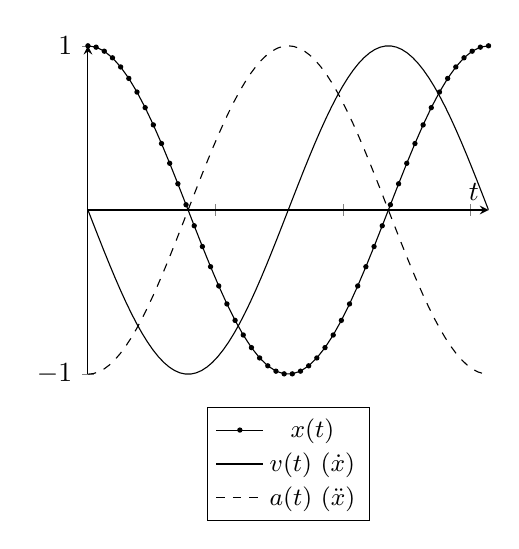
\begin{tikzpicture}
	    \begin{axis}[ xlabel={$t$},
	                    xticklabels={,,},
	                    ytick = {-1, 0, 1},
	                    axis x line = middle,
	                    axis y line = middle,
	                    legend style={at={(0.5,-0.1)},anchor=north},
	                    legend style={font=\small},
	                    width=0.55\columnwidth, ]
	        \addplot[domain=0:2*pi, samples=50, mark=*, mark size=0.75]{ cos(deg(x)) };
	        \addplot[domain=0:2*pi, samples=75]{ -sin(deg(x)) };
	        \addplot[domain=0:2*pi, samples=75, dashed]{ cos(deg(x+pi)) };
	        \legend{$x(t)$, $v(t)$ ($\dot{x}$), $a(t)$ ($\ddot{x}$)}
	    \end{axis}
	\end{tikzpicture}~
	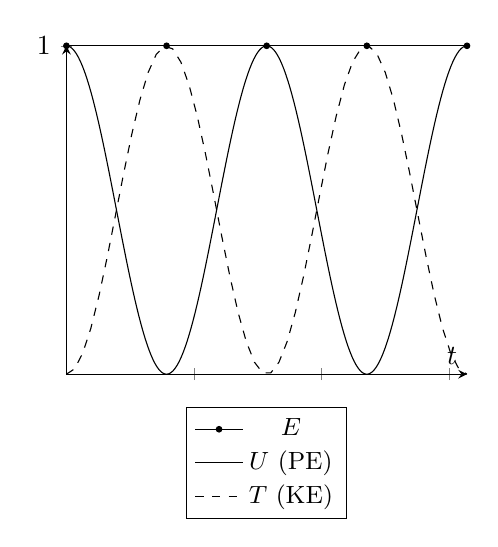
\begin{tikzpicture}
	    \begin{axis}[ xlabel={$t$},
	                    xticklabels={,,},
	                    ytick = {0, 1},
	                    axis x line = middle,
	                    axis y line = middle,
	                    legend style={at={(0.5,-0.1)},anchor=north},
	                    legend style={font=\small},
	                    width=0.55\columnwidth, ]
	        \addplot[domain=0:2*pi, samples=5, mark=*, mark size=1]{ 1 };
	        \addplot[domain=0:2*pi, samples=200]{ (cos(2*deg(x)) + 1)/2 };
	        \addplot[domain=0:2*pi, samples=50, dashed]{( -cos(2*deg(x)) + 1)/2 };
	        \legend{$E$, $U$ (PE), $T$ (KE)}
	    \end{axis}
	\end{tikzpicture}
\end{center} \newpage

\textbf{Small Angle Pendulums}

$\ddot{\theta} = -\frac{g}{l} \theta$ \hfill $\omega = 2 \pi f = \frac{2 \pi}{T} = \sqrt{\frac{g}{l}}$

$\theta = \frac{s}{l} = \omega t + \phi$  \hfill $s$ = arc length, $l$ = length

$s = l \theta = l \left[ \theta_0 \cos(\omega t + \phi) \right]$ \hfill $v_{\text{max}} = \omega l \theta_0$ \hfill $a_{\text{max}} = \omega^2 l \theta_0$

\vspace{-.5em}

\dotfill

\textbf{Damped Oscillators}

$\ddot{x} + 2\zeta \omega_0 \dot{x} + \omega_0^2x = 0$ \hfill $\omega_0 = \sqrt{\frac{k}{m}}$ \hfill $\zeta = \frac{b}{2\sqrt{mk}} = \frac{b}{2m\omega_0}$

$q = \omega_0 \left(-\zeta \pm \sqrt{\zeta^2 - 1} \right)$

\textit{Overdamped} ($\zeta > 1,\ b^2 > 4mk$)
\vspace{-1em}
\begin{center}
	$x(t) = e^{-\omega_0 \zeta t} \left( Ae^{\omega_0 t \sqrt{\zeta^2-1}} + Be^{-\omega_0 t \sqrt{\zeta^2-1}} \right)$
\end{center} \vspace{-1em}

\textit{Critically Damped} ($\zeta = 1,\ b^2 = 4mk$)
\vspace{-1em}
\begin{center}
	 $x(t) = (A + Bt) e^{-\omega_0 t}$
	 
	 $\dot{x} = -A \omega_0 e^{-\omega_0 t} + Be^{-\omega_0 t} - B \omega_0 t e^{-\omega_0 t}$
\end{center} \vspace{-1em}

\textit{Underdamped} ($\zeta < 1,\ b^2 < 4mk$)
\vspace{-1em}
\begin{center}
	$x(t) = \underbrace{ A \overbrace{e^{-\omega_0 \zeta t}}^{ \begin{subarray}{c}\text{decay}\\ \text{envelope}\end{subarray} } }_\text{amplitude}
	\cos ( \underbrace{\overbrace{\omega_0 \sqrt{1 - \zeta^2}}^{ \begin{subarray}{c}\text{angular freq}\\ \text{($\omega_{\text{damped}}$)}\end{subarray} } t + \phi}_\text{phase} )$
	
	\hspace{2em} $A = A_0 e^{-\omega_0 \zeta t}$ \hspace{2.25em} $\omega_{\text{damped}} = \omega_0 \sqrt{1-\zeta^2}$
\end{center} \vspace{-1em}

\begin{center}
    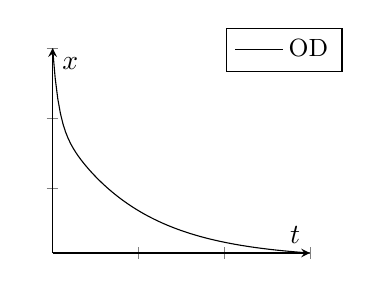
\begin{tikzpicture}
        \begin{axis}[ xlabel={$t$}, ylabel={$x$},
                        xticklabels={,,},
                        yticklabels={,,},
                        axis x line = middle,
                        axis y line = middle,
                        legend style={at={(0.9,1.1)},anchor=north},
                        legend style={font=\small},
                        width=0.4\columnwidth, ]
            \addplot[domain=0:6, samples=100, mark size=1]{ exp(-4*x) * (2*exp(3.464*x) + exp(-3.464*x) ) };
            \legend{OD}
        \end{axis}
    \end{tikzpicture}~
    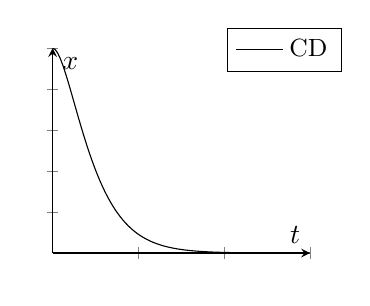
\begin{tikzpicture}
        \begin{axis}[ xlabel={$t$}, ylabel={$x$},
                        xticklabels={,,},
                        yticklabels={,,},
                        axis x line = middle,
                        axis y line = middle,
                        legend style={at={(0.9,1.1)},anchor=north},
                        legend style={font=\small},
                        width=0.4\columnwidth, ]
            \addplot[domain=0:6, samples=100, mark size=1]{ exp(-2*x) * (1 + 2*x) };
            \legend{CD}
        \end{axis}
    \end{tikzpicture}~
    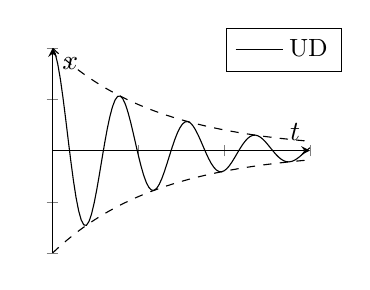
\begin{tikzpicture}
        \begin{axis}[ xlabel={$t$}, ylabel={$x$},
                        xticklabels={,,},
                        yticklabels={,,},
                        axis x line = middle,
                        axis y line = middle,
                        legend style={at={(0.9,1.1)},anchor=north},
                        legend style={font=\small},
                        width=0.4\columnwidth, ]
            \addplot[domain=0:6, samples=100]{ exp(-0.4*x) * cos(deg(3.98 * x)) };
            \addplot[domain=0:6, samples=100, dashed]{ exp(-0.4*x) };
            \addplot[domain=0:6, samples=100, dashed]{ -exp(-0.4*x) };
            \legend{UD}
        \end{axis}
    \end{tikzpicture}
\end{center} \vspace{-2em}

\dotfill

\textbf{Driven Oscillators and Resonance}

$m\ddot{x} = -kx - b\dot{x} + F_0 \cos(\omega t)$ \hfill $\Rightarrow$ \hfill $\ddot{x} + 2 \zeta \omega_0 \dot{x} + \omega_0^2 x = \frac{F_0}{m} \cos(\omega t)$

$A = \frac{F_0}{m} \frac{1}{\sqrt{(\omega_0^2 - \omega^2)^2 + 4\omega_0^2\omega^2\zeta^2}}$ \hfill $\phi = \tan^{-1} \left( \frac{2\omega_0 \omega \zeta}{\omega_0^2 - \omega^2} \right)$

$\omega_r = \omega_0 \sqrt{1- 2 \zeta^2}$ \hfill $\zeta < \frac{1}{\sqrt{2}}$ \hfill $\zeta \ll 1, \omega_r \approx \omega_0$

$\lim\limits_{\omega \rightarrow 0} \phi = 0$ (low $\omega$) \hfill $\lim\limits_{\omega \rightarrow \omega_0} \phi = \pi/2$ ($\omega = \omega_0$) \hfill$\lim\limits_{\omega \rightarrow \infty} \phi = \pi$ (high $\omega$) \vspace{-2em}

\begin{center}
    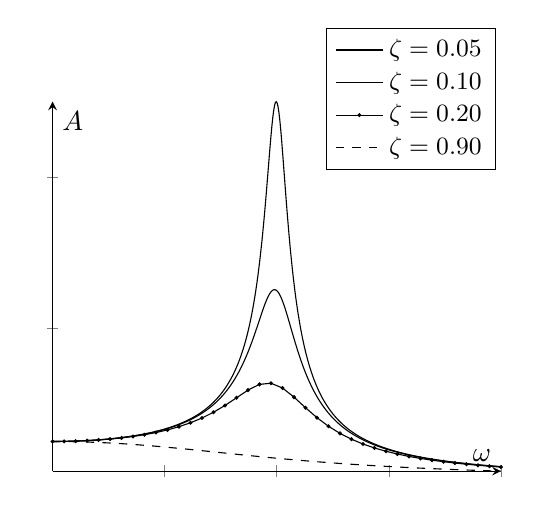
\begin{tikzpicture}
        \begin{axis}[ xlabel={$\omega$}, ylabel={$A$},
            xticklabels={,,},
            yticklabels={,,},
            axis x line = middle,
            axis y line = middle,
            legend style={at={(0.8,1.2)},anchor=north},
            legend style={font=\small},
            width=0.6\columnwidth, ]
            \addplot[domain=0:4, samples=500]{ 1 / sqrt( (4-x^2)^2 + 16*x^2*0.05^2) };
            \addplot[domain=0:4, samples=400]{ 1 / sqrt( (4-x^2)^2 + 16*x^2*0.1^2) };
            \addplot[domain=0:4, samples=40, mark size=.5, mark=*]{ 1 / sqrt( (4-x^2)^2 + 16*x^2*0.2^2) };
            \addplot[domain=0:4, samples=40, dashed]{ 1 / sqrt( (4-x^2)^2 + 16*x^2*0.9^2) };
            \legend{$\zeta = 0.05$, $\zeta = 0.10$, $\zeta = 0.20$, $\zeta = 0.90$}
        \end{axis}
    \end{tikzpicture}~
    \includegraphics[width=0.5\columnwidth]{Figures/res.png}
\end{center} \vspace{-1em}

$E = \frac{1}{2} kA^2 e^{-2 \omega_0 \zeta t} = \frac{1}{2} kA^2e^{-bt/m}$ \hfill $\omega = \omega_0 \approx \omega_r$ at $\Delta \phi = \frac{\pi}{2}$ \hspace{1em}


\end{document}

















